% Use only LaTeX2e, calling the article.cls class and 12-point type.

\documentclass[12pt]{article}

% Users of the {thebibliography} environment or BibTeX should use the
% scicite.sty package, downloadable from *Science* at
% www.sciencemag.org/about/authors/prep/TeX_help/ .
% This package should properly format in-text
% reference calls and reference-list numbers.

\usepackage{scicite}
\usepackage{xcolor}
\usepackage[utf8]{inputenc} %unicode support
\def\includegraphic{}
\def\includegraphics{}
\usepackage{graphicx}
\usepackage{subcaption}
% Use times if you have the font installed; otherwise, comment out the
% following line.

\usepackage{times}

% The preamble here sets up a lot of new/revised commands and
% environments.  It's annoying, but please do *not* try to strip these
% out into a separate .sty file (which could lead to the loss of some
% information when we convert the file to other formats).  Instead, keep
% them in the preamble of your main LaTeX source file.


% The following parameters seem to provide a reasonable page setup.

\topmargin 0.0cm
\oddsidemargin 0.2cm
\textwidth 16cm 
\textheight 21cm
\footskip 1.0cm


%The next command sets up an environment for the abstract to your paper.

\newenvironment{sciabstract}{%
\begin{quote} \bf}
{\end{quote}}


% If your reference list includes text notes as well as references,
% include the following line; otherwise, comment it out.

\renewcommand\refname{References and Notes}

% The following lines set up an environment for the last note in the
% reference list, which commonly includes acknowledgments of funding,
% help, etc.  It's intended for users of BibTeX or the {thebibliography}
% environment.  Users who are hand-coding their references at the end
% using a list environment such as {enumerate} can simply add another
% item at the end, and it will be numbered automatically.

\newcounter{lastnote}
\newenvironment{scilastnote}{%
\setcounter{lastnote}{\value{enumiv}}%
\addtocounter{lastnote}{+1}%
\begin{list}%
{\arabic{lastnote}.}
{\setlength{\leftmargin}{.22in}}
{\setlength{\labelsep}{.5em}}}
{\end{list}}


% Include your paper's title here

\title{Leveraging insurance customer data to characterize socioeconomic indicators of Swiss municipalities \\ \vspace{3mm} Response to reviewers} 


% Place the author information here.  Please hand-code the contact
% information and notecalls; do *not* use \footnote commands.  Let the
% author contact information appear immediately below the author names
% as shown.  We would also prefer that you don't change the type-size
% settings shown here.

\author
{Lorenzo Donadio$^{1}$,  Rossano Schifanella$^{2}$, Claudia R. Binder$^{1}$ \\ Emanuele Massaro $^{1\ast}$\\
\\
\normalsize{$^{1}$HERUS Lab, École polytechnique fédérale de Lausanne, Switzerland}\\
\normalsize{$^{2}$University of Turin, ISI Foundation, Turin, Italy}\\
\\
\normalsize{$^\ast$To whom correspondence should be addressed; E-mail:  ema.massaro@gmail.com.}
}

% Include the date command, but leave its argument blank.

\date{}



%%%%%%%%%%%%%%%%% END OF PREAMBLE %%%%%%%%%%%%%%%%



\begin{document} 

% Double-space the manuscript.

\baselineskip24pt

% Make the title.

\maketitle 



% Place your abstract within the special {sciabstract} environment.

\begin{sciabstract}

\end{sciabstract}


\section*{Comments from Associate Editor}



The reviewers agree that the data set used in the paper is interesting and there is potential value in using it to understand and predict socio-economic status. However, there are several weaknesses that make the paper unfit for publication at its current state.

I encourage the authors to address and/or respond to all the reviewers' comments. In particular, there are three main areas of improvement:

1. Reviewer 1 points out that most of the results seem trivial. The authors should expand the discussion to further explain the insights obtained from the results or expand their analysis. Along these lines, reviewer 2 points out that the claim about the possible application of their methods for geographical fine-grained contexts is not supported by the results. Could the authors actually show that their method could be applied for a more fine-grained measurements?

2. As reviewer 1 points out, the authors need to show the value added by their data/method by comparing its performance to some baselines.

3. There are a number of technical weaknesses pointed out by reviewer 2 that would need to be addressed for the paper to be published (e.g a systematic comparison of performance across different regions, discussion on effect sizes, etc.)

\vspace{1cm}
Dear Editor,

Our thanks to you and the reviewers for your positive comments and constructive suggestions. We have revised the manuscript addressing all the editorial comments. Please find the list of all the changes to the manuscript in our point-by-point response below. The original referees’ comments are in bold. We share our findings and analysis with you and the reviewers in a public repository~\footnote{https://github.com/emanuelemassaro/insurancepaper}.\\

In this document, we tried to answer to all the comments made by reviewers by explaining point to point the validity of our results and methodology.

Sincerely yours,

Lorenzo Donadio, Rossano Schifanella, Claudia R. Binder and Emanuele Massaro.



\section*{Comments from Reviewers:}

\subsection*{Reviewer 1}

\textbf{This is an interesting paper in which the authors study the explanatory power of variables from an insurance company to explain some socio-demographic indicators of Swiss municipalities. Because of the limitations of the indicators, the authors are only able to study 170 points (municipalities) using 34 variables constructed from the insurance data. In both the OLS, SLM and GWR the authors find that a small number of variables are important in the models.\\I see the value of the use of a new source of data (insurance) to understand SES (socio-economic status), however, most of the results found are really trivial (see table 6): work related to number of unemployed customers (!), fraction of foreigns related to fraction of foreigners (in costumers), cars per 1000 inhabitants correlated to the number of unemployed customers, etc.\\Even for the example discussed at the end (transportation), the results are somehow trivial: fraction of commuters using public transportation seems to be highly dependent on the number of people owning a house or the percentage of insured cars.}

We thank the reviewer for appreciating our work and his interesting comments. From our analysis is possible to find some relations between the extracted features from the insurance dataset and the socio-economic indicators that can appear trivial. For instance, we can observe those \emph{obvious} relationships:

\begin{itemize}
\item the target variable $p_1$ : \emph{Fraction of foreigners} and the aggregated feature $f4$ : \emph{Fraction of foreigners}
\item the target variable $p_2$ : \emph{Fraction of beneficiaries of the social assistance} and the aggregated feature $f1$ : \emph{Unemployment rate}
\item  the target variable $w_1$ : \emph{Unemployment rate} and the aggregated feature $f1$ : \emph{Unemployment rate}
\item  the target variable $w_2$ : \emph{Unemployment rate between women} and the aggregated feature $f1$ : \emph{Unemployment rate}
\end{itemize}

We tried to see the added values of such features. In predicting those variables we remove the aforementioned \emph{trivial} features. We also removed the features $f1$ : \emph{Unemployment rate} to predict the variable $t_1$: cars per 1000 inhabitants and we removed the features $f3$ : \emph{Fraction of owners (house)} and $f20$: \emph{Percent of insured cars}  to predict the variable $t_2$: \emph{Fraction of commuters using public transportation}. In the Section 8.1 of the shared notebook and in~\figurename~\ref{fig:deltaR2}.


\begin{figure}[h!]
    \centering
    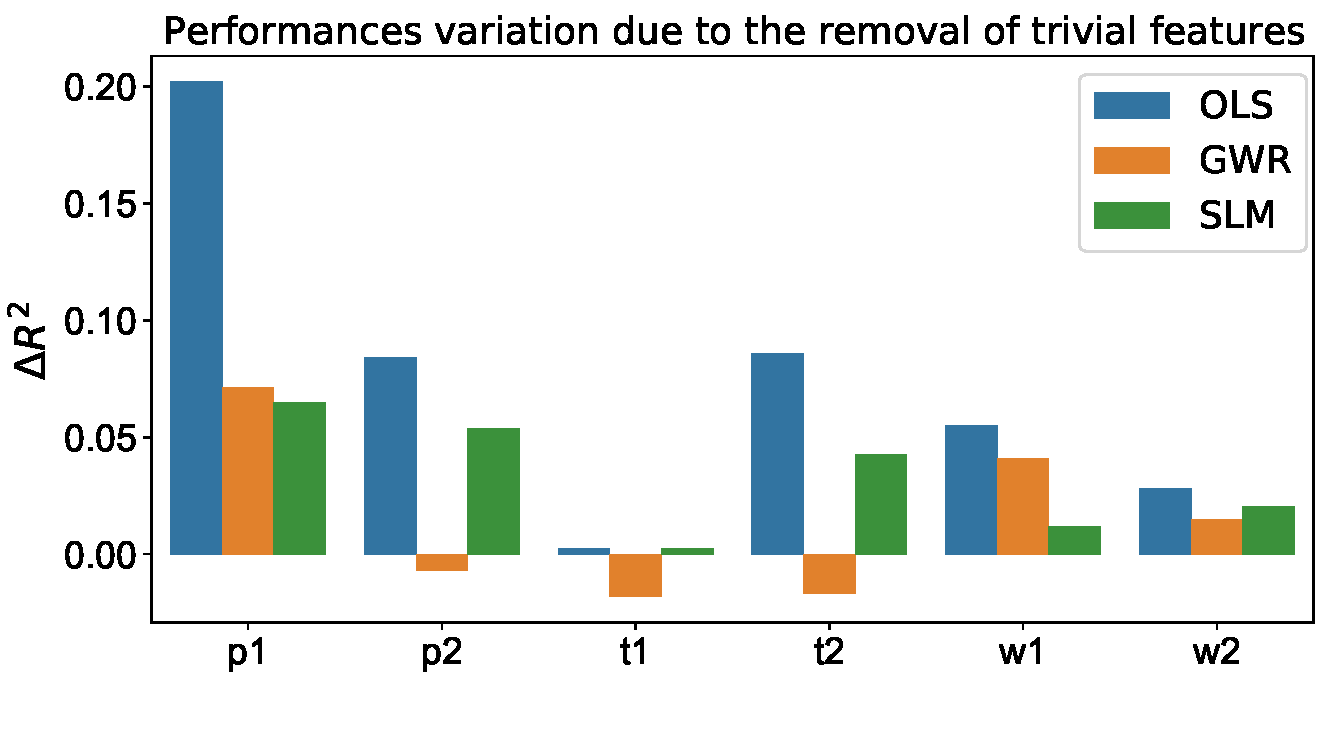
\includegraphics[width=1\linewidth]{figures/deltaR2_new.pdf}
\caption{Variation of the performance of the models in predicting the aforementioned target variables without the use of \emph{trivial} features.}
\label{fig:deltaR2}  
\end{figure}

In~\figurename~\ref{fig:deltaR2} we can see that only the OLS model largely suffers of the exclusion of the trivial target variables. For the GWR we observe an average difference of the model's performance of 0.014, while this difference is 0.032 for the SLM.

We believe that those relationships can give more credit to our assumptions and to our work because it means that the dataset we are observing is representative of the Swiss population.  In the manuscript we also emphasize the fact that there is a strong relationship between fraction of commuters using public transportation and the number of people owning a house.  This point has attracted a lot of attention in the scientific community as, for instance, reported in a study in the United States~\cite{zhang2018exploring}.

On the other side, there are some target variables that they are predicted by \emph{non trivial} features such as
\begin{itemize}
\item 'Building area (\%)'
\item 'Green area (\%)'
\item 'Average area per inhabitant in square meters'
\item 'Municipal debt' 
\item 'Fraction of investment in culture
\item 'Cars per 1000 inhabitants'
\item 'Fraction of commuters using public transportation'
\end{itemize}



\vspace{1cm}
\textbf{a) Spatial regressions are used, but the data (see Figure 1) is very patchy geographically and I wonder whether even makes sense to use spatial regressions.}

We thank a lot the reviewer for this comment.  In the research we made use of geographical regression models for different reasons. First, because the Swiss territory is characterized by heterogeneous administrative units (cantons) and by different languages (Swiss French, Swiss German and Swiss Italian). 

Moreover, spatial analysis does not apply only to contiguous spatial units but also on spatial relationships that involve distance, for example. The main point of using spatial regressors is when the residuals of the regression are spatially correlated, against the null of a random distribution over space.

We  checked the residuals for normality and apply the same methodology already proposed~\footnote{http://darribas.org/} as shown in Section 8.2 of the shared notebook.

\begin{table}[h!]
\centering
\caption{Residuals of the Moran's i in respect to the global model}
\label{tab:residuals}
\begin{tabular}{ccccc}
\hline
   & $I_{res}$  & p-value$_{res}$ & $I_{var}$  & p-value$_{var}$ \\
\hline
p1	&0.2893	&0.0001	&0.3675	&0.0001  \\
p2	&0.1908	&0.0007	&0.4483	&0.0001 \\
t1	&0.1051	&0.1323	&0.1733	&0.0090\\
t2	&0.3604	&0.0001	&0.4179	&0.0001\\
w1&	0.2519	&0.0001	&0.4714	&0.0001\\
w2&	0.2541	&0.0001	&0.4457	&0.0001\\
s1&	0.2024	&0.0003	&0.3400	&0.0001\\
s2	&0.1841	&0.0020	&0.2335	&0.0006\\
h1	&0.2405	&0.0005	&0.2959	&0.0001\\
h2&	0.2556	&0.0001	&0.4388	&0.0001\\
e1&	0.2368	&0.0002	&0.2951	&0.0001\\
e2&	0.1194	&0.0636	&0.5087	&0.0001
\end{tabular}
\end{table}

In Table~\ref{tab:residuals} we report four values for each target variables:
\begin{itemize}
\item  $I_{res}$: Moran's I of the residuals of the Ordinary Linear Squares (OLS) regression model;
\item $P-value_{res}$: p-value based on permutations (one-tailed) null: spatial randomness alternative: the observed I is extreme if it is either extremely greater or extremely lower than the values obtained based on permutations;
\item $I_{var}$: Moran's I of the normalized target variables;
\item $P-value_{var}$: same of before but for the target variables.
\end{itemize}

The results in Table~\ref{tab:residuals} are a series of statistics that test whether the residuals of the regression are spatially correlated, against the null of a random distribution over space.  If the latter is rejected a key assumption of OLS, independently distributed error terms, is violated. Depending on the structure of the spatial pattern, different strategies have been defined within the spatial econometrics literature to deal with them~\footnote{https://sgsup.asu.edu/geodacenter-redirect}. The main summary from the diagnostics for spatial dependence is that there is clear evidence to reject the null of spatial randomness in the residuals, hence an explicitly spatial approach is warranted.

\vspace{1cm}
\textbf{b) The models do not allow to know what is the added value of the insurance data to simple statistics. I suggest the authors use simple fixed factors to control for the specific Swiss region or for total population to see what is the added value of insurance-related features to simple models. The reader need a simple baseline to understand how much value the new features introduce.}

We thank again the reviewer for this important comment. We agreed that a baseline is important to understand the added value of such dataset. For this reason, we designed a baseline model that consists in using as features the census data. In the baseline model, we predict each target variable by considering all the target variables except the one we want to predict. For instance for predicting the variable $p_1$, we use the variables $p_2$, $t_2$,....,$e_2$.  In~\figurename~\ref{fig:deltaPer} we report the comparison between the baseline and the insurance data models for each model. In~\figurename~\ref{fig:deltaPer} we compute $\Delta R^2$ as the difference of the performance between the models with insurance data and the baseline. 

\begin{figure}[h!]
    \centering
    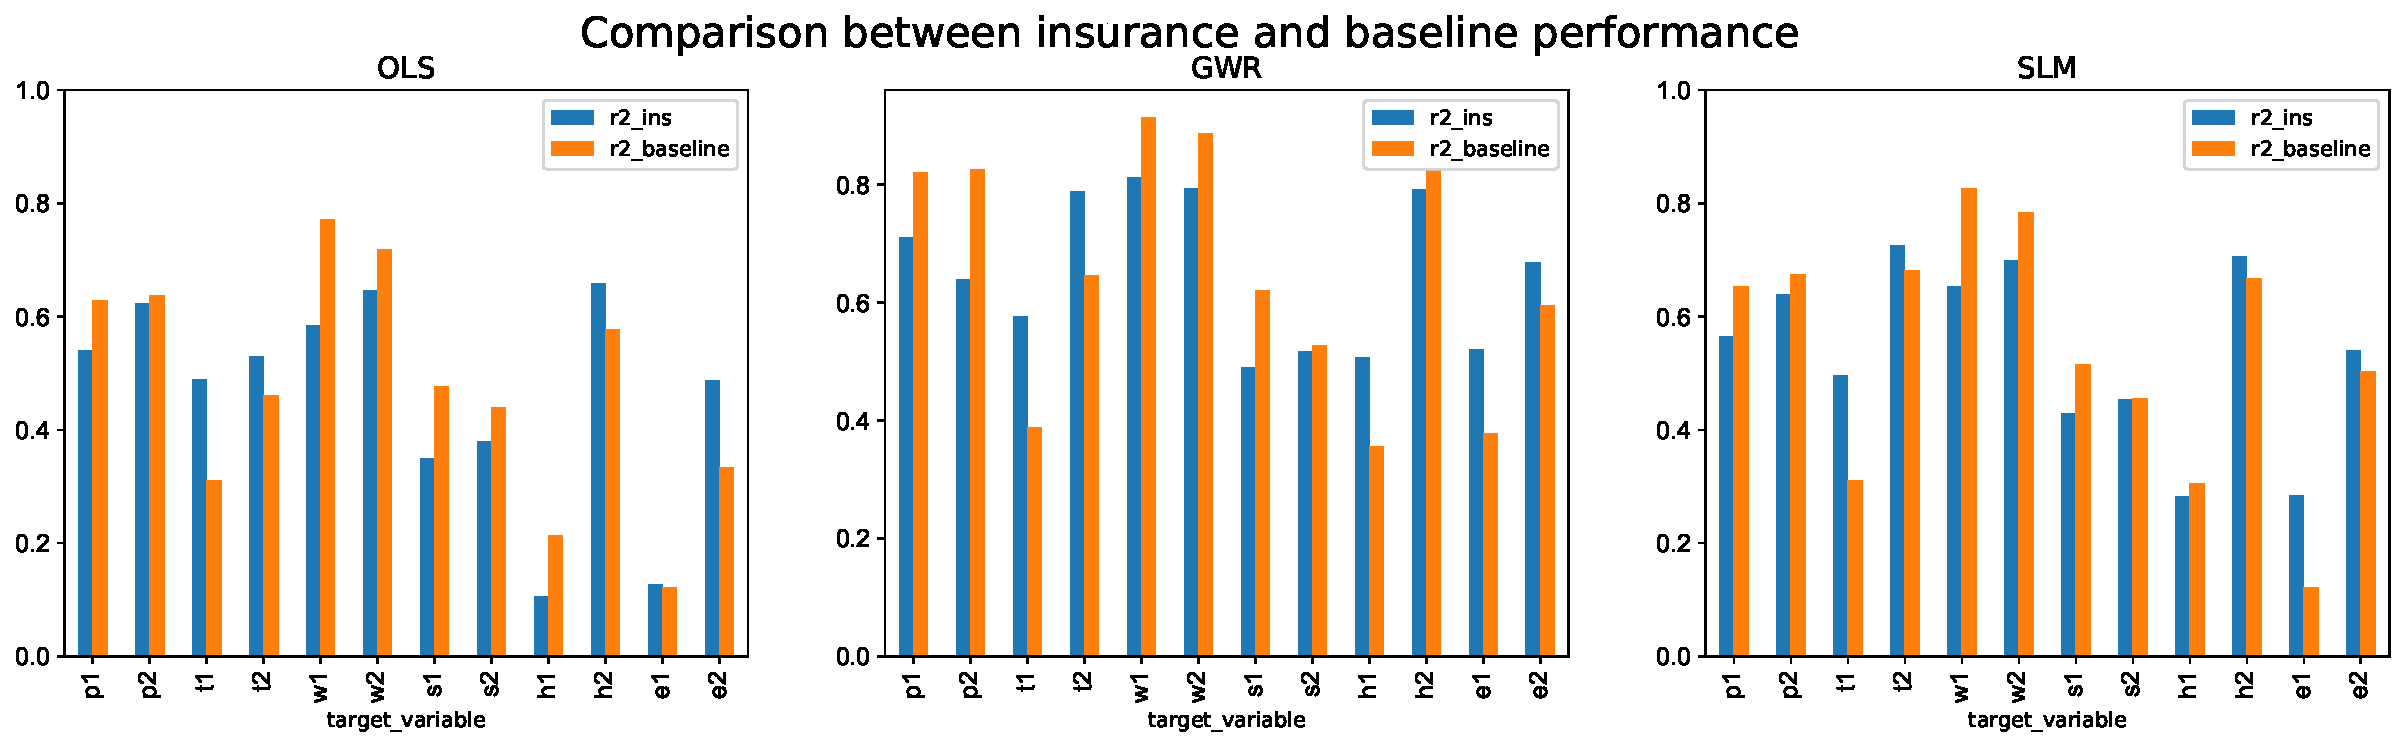
\includegraphics[width=1\linewidth]{figures/comparison0.pdf}
\caption{Variation of the performance of between in terms of $R^2$. Here we compute the difference between the models with the insurance data and the baseline for the different models.}
\label{fig:baseline}  
\end{figure}


\begin{figure}[h!]
    \centering
    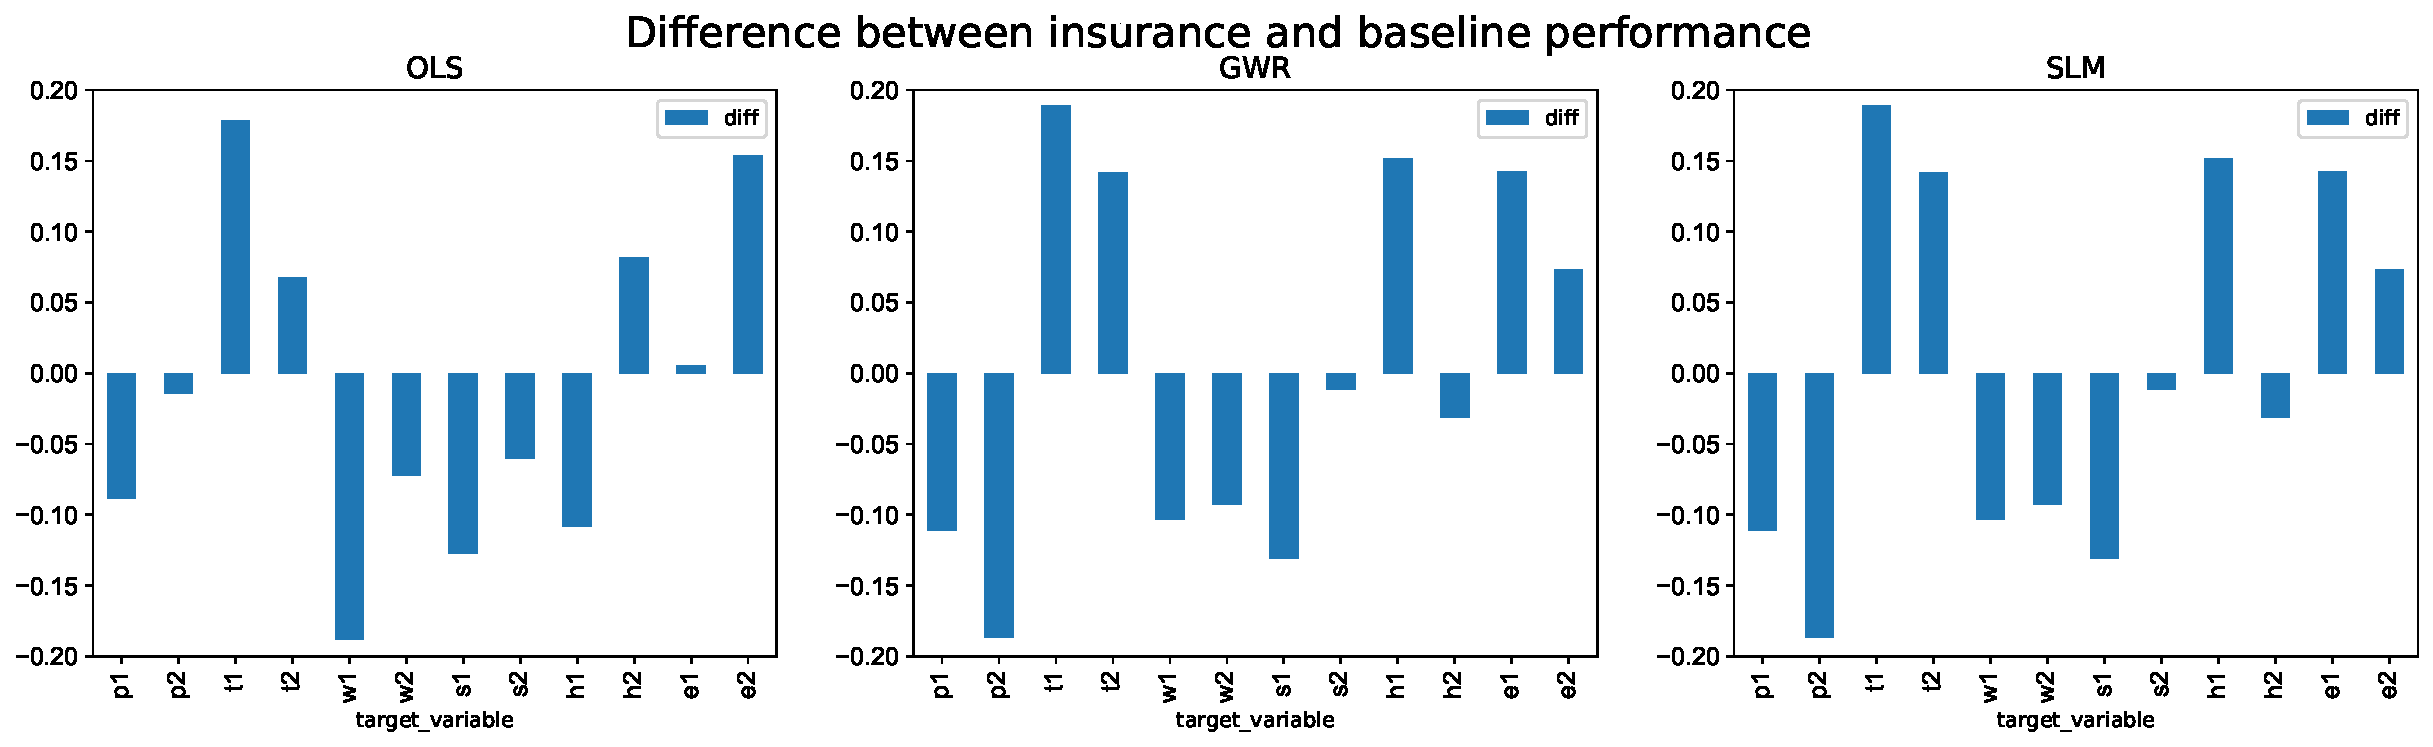
\includegraphics[width=1\linewidth]{figures/comparison.pdf}
\caption{Variation of the performance of between in terms of $R^2$. Here we compute the difference between the models with the insurance data and the baseline for the different models.}
\label{fig:deltaPer}  
\end{figure}

From \figurename~\ref{fig:baseline} and \figurename~\ref{fig:deltaPer}  we can observe that the spatial models work better than the standard OLS model even in this case. 

\begin{figure}[h!]
    \centering
    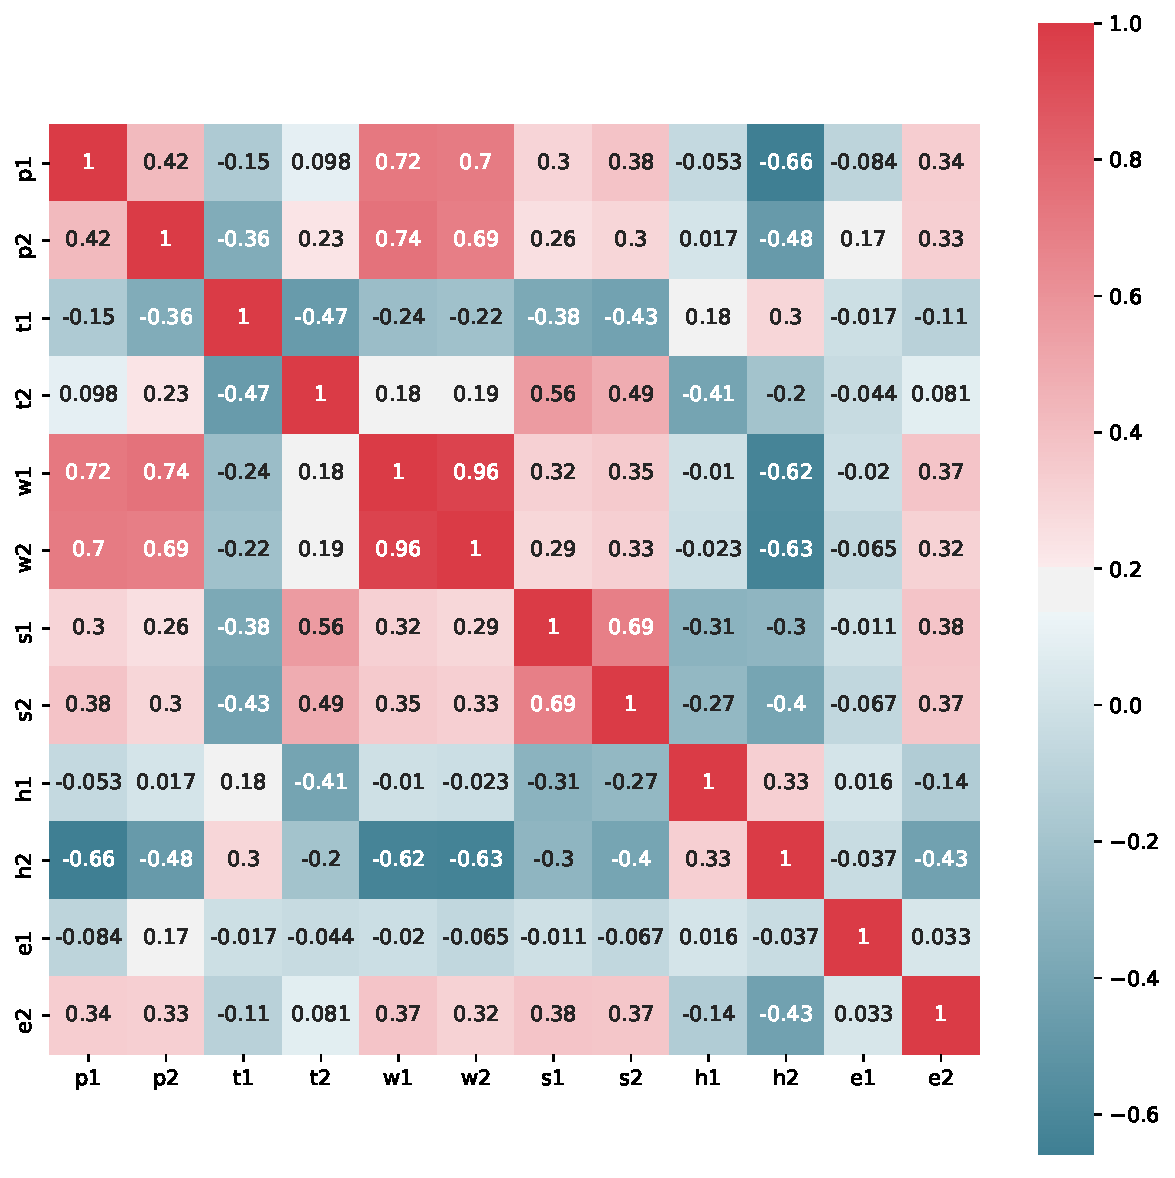
\includegraphics[width=.7\linewidth]{figures/correlationTargets.pdf}
\caption{Correlation matrix of the target variables used as features of the baseline models.}
\label{fig:corrTarg}  
\end{figure}

We can also observe that the GWR baseline perform better than the one that use the insurance data, especially for the variables that are well predicted (see $p_1$, $p_2$, $w_1$, $h_2$). However,  in average, the difference between the two models in $0.019$ for the global model and $0.0019 $ for the GWR. The better performance is given by the fact that the data comes from the same source, it was collected the same way and some indicators are really similar to each other.  In~\figurename~\ref{fig:deltaPer} we report the correlation matrix for the target variables from the census. We can notice that the variable that are well predicted such as $p_1$, $p_2$, $w_1$, $w_2$ show a strong correlation with other variables: this is why the baseline model can predict  well some variables.


We would like to stress again that our goal is to overcome the use of official statistical data in order to show the effectiveness of alternative dataset and we want to put ourselves in a scenario where no census data is available.

\subsection*{Reviewer 2}

\textbf{This paper explores the potential for using home and vehicle insurance data to predict socioeconomic features of geographical regions. It builds on extensive prior work in the domain of using observation data to understand the socioeconomic and demographic features of regions and introduces a new comparatively rich dataset while also employing methods , sensitive to spatial-autocorrelations, that are relatively novel to the domain. Below, I list the key strengths and weaknesses of the work as well specific comments to the authors.\\Key Strengths\\1. The exploration of a novel dataset source for the important application of efficiently and accurately measuring socioeconomic indicators for geographic regions. This dataset is generally richer and more meaningful than other observational datasets that have been used for the same purpose (Ex: call detail records, social media data such as Tweets etc.)\\2. The authors employ techniques that are sensitive to geographic correlations in socioeconomic features and also leaves room for regional idiosyncrasies\\3. The authors explore the predictive power of their observational features in different regions and make an, somewhat rudimentary, attempt to account for those differences.}

We thank the reviewer for appreciating our work. 

\vspace{1cm}
\textbf{Key Weakness}\\
\textbf{1. The authors' claim about the validity and usefulness of their approach to contexts where official statistics are not available, in particular small geographic regions such as neighborhoods, is not explored or supported in this paper.}

We thank a lot the reviewer for this comment. We explained better the fact that in the next steps we would like to test the validity of this modus operandi also for neighborhoods and smaller urban areas. Indeed in this paper we did not demonstrate this possibility. Together with the notebook that contains all the analysis we made for this revision, we also enclosed a two .pdf file that show the differences between the original and the final manuscript in which we addressed all the comments made by the reviewer.

\vspace{1cm}
\textbf{2. The paper lacks clarity, especially the results section, and in one particular case seems to be missing a figure}\\
We thank a lot again the reviewer for this comment that helped us a lot to improve the manuscript. For this reason we revised many parts and especially the results section as suggested by the reviewer.


\vspace{1cm}
\textbf{3. Despite having made an initial foray into understanding under what circumstances (geographic, economic) this data and methods employed would perform better or worse, no systematic exploration or discussion is included. Such an analysis would have been significant contribution.}
\\
We thank again the reviewer for this comment. We changed and revised the text according to this comment, explaining that we would like to try this methodology also for predicting the socio-economic status of neighborhoods and smaller urban areas. In this paper, we did not find any patterns that suggest a clear correlation between socio-economic or geographical circumstances our models perform better. We presented a detailed answer to this point in the next section (Point 8) and with reference to the notebook we shared.

\vspace{1cm}
\textbf{Specific Comments\\1. The authors claim in the abstract and the conclusion that their methods may be useful for more geographically fine-grained contexts such as city neighborhoods, a fact that they contradict in their discussion of limitations. Given that their analysis has been conducted at a coarse grained level of municipalities and no attempt has been made to establish mechanisms of how behaviors observed through insurance data are related to socioeconomic indicators as well as evaluating the level of representativeness of the data beyond population counts, I believe this claim is for the most part unjustified. Blumenstock et al. (2015) is a good example of how the first part of the above challenge has been met with a mixed method approach. This mechanistic linkage between the observed measures and the predicted the socioeconomic indicators is also crucial for an understanding of how geographically and temporally stable the observed correlations are (consider Google Flu Trends)
}
\\
We agreed with the reviewer. Indeed, in this manuscript we did not prove that this modus operandi could work well also on more geographically fine-grained contexts. What we would like to say is that, as future steps, we would like to test our models also on  big city neighborhoods such Geneva or Zurich. Thanks to this comment we revised our manuscript in order to make clear that this analysis would part of a next research.


\textbf{2. The authors should consider adding a discussion on how and why the original features listed in Table 3 were selected. It would strengthen their arguments if these features had been derived based on prior literature as opposed to in a ad-hoc manner}\\
We thank a lot the reviewer for this comment that helped us to improve the manuscript. 
\begin{table}[h]
\tiny
\centering
\caption{From data at ZIP code level to features at municipality leve.}
\label{tab:insurancedata}
\begin{tabular}{l|l|p{6.5cm}|p{3.5cm}}
Catergory							& Variable Name 						& Extracted feature 					& Motivation                   							\\
\hline
\hline
Demographic 					& Nmbr               						& to count Market share $f6$   and Number of customers divided by total customers $f8$ 							&                   			\\ \hline
										& JobState           						& Unemployment rate $f1$        &                            										\\ \hline
										& Civil              							& None                                         &  We considered the number of children       \\ \hline
										& Gender             						& Fraction of women $f7$          &                            \\ \hline
										& YearOfBirth                              & Average age $f2$                    &                            \\ \hline
										& Own/Rent           						& Fraction of owners $f3$          &                 \\ \hline
										& Lang  (Speaking language)     & None                                           & We considered the number of foreigners \\ \hline
										& Nation             						&  Fraction of foreigners $f4$     &                           \\					 \hline					
										&ZIP                & None                                       & We are interested in the local muncipality                    \\ \hline
									    &Children\_0-26     & Average number of customers with at least one child $f5$                                            &       \\ \hline \hline
Cars &Car1\_Canton*      & None                         & Not relevant for this study                           \\ \hline
&Car1\_Brand*       & None                                         & We considered the price and the cylinder capacity as proxy for the car type                           \\ \hline
&Car1\_Price*       & $f9$, $f10$  Average price, 95th percentile                                  &                           \\ \hline
&Car1\_Year         & $f11$, $f12$ Average year of the car  and 5th percentile year of the car                   &         \\ \hline
&Car1\_ccm*         & $f13$, $f14$ Average CCM of the car and 95th percentile CCM of the car       &                           \\ \hline
&Car1\_ClaimsCt5Y*  & $f15$, $f16$ Average number of claims per car  and 95th percentile number of claims of the car   &  \\ \hline
&Car1\_ClaimsSum5Y* & $f17$, $f18$ Average sum of claims of the car and 95th percentile number of price of the car &                             \\ \hline
&Car\_Premium       & $f19 $Average premium of the car            &                            \\					     \hline                             								    
&overall & $f20$ Percent of insured cars   								   &                            \\					     \hline  \hline
Housing&HH\_Zip            & None                               & Not relevant                     \\ \hline
&HH\_Ins\_Sum       & None           & We used insured premium                          \\ \hline
&Stand\_of\_furn    & $f21$: Average class of furniture and $f22$: 95th percentile class of furniture    &  \\ \hline
&Rooms              & $f23$: Average number of rooms and $f24$: 95th percentile number of rooms       &                        \\ \hline
&Build\_Zip         & None                            & Not relevant                     \\ \hline
&Build\_Ins\_Sum    & $f25$: Average building insured sum and $f26$: 95th building insured sum        &                           \\ \hline
&Year\_ofcontrs     & $f27$: Average building year of Construction and $f28$: 5th percentile building year of construction              \\ \hline
&Type               & $f29$: Average type of building                                    &                        \\ \hline
&HHaB\_ClaimsCt5Y   & $f30$: Average number of claims per building    &    \\ \hline
&HHaB\_ClaimsSum5Y  & $f31$: Average sum of claims per building and $f32$: 95th sum of claims per building  &                           \\ \hline
&HH\_and\_Bld\_Prem & $f33$: Average Insured Premium and $f34$: 95th sum of insured premium                              & String        
\end{tabular}
\end{table}
Our future selection is data-driven and not theoretical-driven. In particular we started in analyzing the available information of our dataset and reported in Table 2 of the manuscript. From the information of the original dataset we wanted to extract all the possible information. We tried to take into account all the variables and we also removed overlapping or unessential information. In Table~\ref{tab:insurancedata} we report the interplay between the original dataset and the extracted features: in table we reported the explanation of why a variable has not been selected. 



Thanks to this approach we were able to extract and aggregate all the available information for each municipality starting from the single costumer's information. We would like to say that we did not make any bottom-up consideration of the use of the data that we took into consideration but we used a complete data-driven top-down approach (also in the subsequent feature selection step).
\\

\textbf{3. In both regression methods, the authors have chosen to estimate certain parameters that apply across all models (dependent variables) and all cities (In SLM, \# nearest neighbors and the bandwidth b in GWR). This was likely done to simplify the analysis. How would this compare in terms of performance to the approach where these parameters are estimated separately for each dependent variable?. It would also generate an interesting if somewhat secondary result on the extent to which these different dependent variables are geographically correlated.}
\\

We would like to thank the reviewer for this comment and we would like to answer at this point. Probably we did not explain well in the manuscript and we tried to better explain this point also in the manuscript. Let us say that for the SLM the number of nearest neighbors is only dependent on the geometry and for this reason it is only determined once. In the SLM we introduce the space  by ``spatially laggin'' one of the explanatory variables. In a Spatial Lag Model (SLM), the first and most straightforward way to introduce space is by ``spatially lagging'' the dependent variable. One must then treat it as an endogenous variable, this is known as a Spatial Autoregressive Model. Formally. This can be expressed in matrix notation, as follows~\cite{anselin2001spatial}:
 \begin{equation}
 y = \alpha + \beta X+\lambda W y + \epsilon
 \end{equation}

where $y$ is the vector of observations on the dependent variable, $X$ is the matrix of observations on the exogenous variables, $W$ is the spatial weighting matrix of known constants, $\beta$ is the vector of regression parameters and $\lambda$ is the scalar autoregressive parameter. The variable $Wy$ is typically known as the spatial lag of $y$. The weighting scheme will determine how the spatial dimension of the problem is incorporated in the model. A k-nearest neighbors (KNN) scheme was chosen, and the number of nearest neighbors to include in the scheme was optimized by maximizing the average $R^2$ over all the dependent variables and found to be equal to ten neighbors. This particular model does violate some of the assumptions of OLS, since it includes an endogenous variable on the right-hand side of the equation. To obtain reliable coefficients the PySAL package was used ~\cite{pysal2007}.

For the GWR the bandwidth does depend on the geometry but also on the distribution of the target variable, and so we select one bandwidth per target variable (for all municipalities)~\cite{oshan2019mgwr}.  The general formula for a GWR is that one regression is calculated for each point using spatial weights.

\begin{equation}
\label{eq:weights}
y_i=\beta_{0i}+ \sum _{j=1}^{m} \beta _{i,j}X_{i,j} + \epsilon_i.
\end{equation}

The index $i$ indicates the location of the city of interest. GWR basically fits a set of $\beta$ coefficients for each location:
\begin{equation}
\beta_i=(X^TW_iX)^{-1}X^TW_iy,
\end{equation}
where $W_i$ is the diagonal matrix of the spatial weights, unique to location $i$. There are various schemes for calculating the weights, nearest neighbors, cubic or exponential kernels.  The weights are computed by the following:
%
\begin{equation}
w_{i,j}=\exp(-0.5\frac{d_{i,j}^{2}}{b}),
\end{equation}
%
where $d_{ij}$ is the Euclidean distance between municipality $i$ and $j$ and $b$ is the bandwidth of the kernel that has to be chosen. For each municipality we calculate a vector of weights and then regress using the final formula (whether linear or with interactions), in order to estimate all indicators for each municipality. The parameters form the GWR will be the focus of some analysis because of the non-stationarity of the problem it is interesting to explore how the influence of certain explanatory variables changes from city to city and whether there are underlying tendencies. 
%
We estimated a fixed bandwith for every city and every model. The optimum bandwidth can be estimated by minimizing an information criterion; In practice, a corrected version of the AIC is used, which unlike basic AIC is a function of sample size~\cite{hurvich1998smoothing}.  Thus for a GWR model with a bandwidth $b$, the $AIC_c$ is given by:
%
\begin{equation}
AIC_{c}=2n\ln{\hat{\sigma}}+n\ln{2\pi}+n\frac{n+tr(S)}{n-2-tr(S)},
\end{equation}
%
where $\hat{\sigma}$ is the estimated standard deviation of the residuals; $n$ is the number of observations and $tr(S)$ is the trace of the hat matrix $S$. The hat matrix is the projection matrix from the observed $y$ to the fitted values $\hat{y}$~\cite{hoaglin1978hat}. Each row of the hat matrix is calculated as follows:
%
\begin{equation}
row_i=X_i(X^{T}W_iX)^{-1}X^{T}W_i
\end{equation}


\textbf{4. It wasn't immediately clear why the variable "market share" had been selected for the models. The discussion section does explain that this variable in fact correlates with the urban-rural divide. I would think that this phenomenon would be quite readily available in official statistics. In addition, the explanation in the discussion indicates that the nature of the relationship between the market share and prevalence of cars is quite idiosyncratic to the particular insurance company whose data is being used. Thus I'm not sure what value this variable would beyond a generic "urban-rural" or population density variable that can be derived more accurately from other sources.}
\\
We thank the reviewer for this comment: we addressed this point also in the manuscript and in Section 8.3 of the shared notebook. 
\begin{figure}[h!]
    \centering
    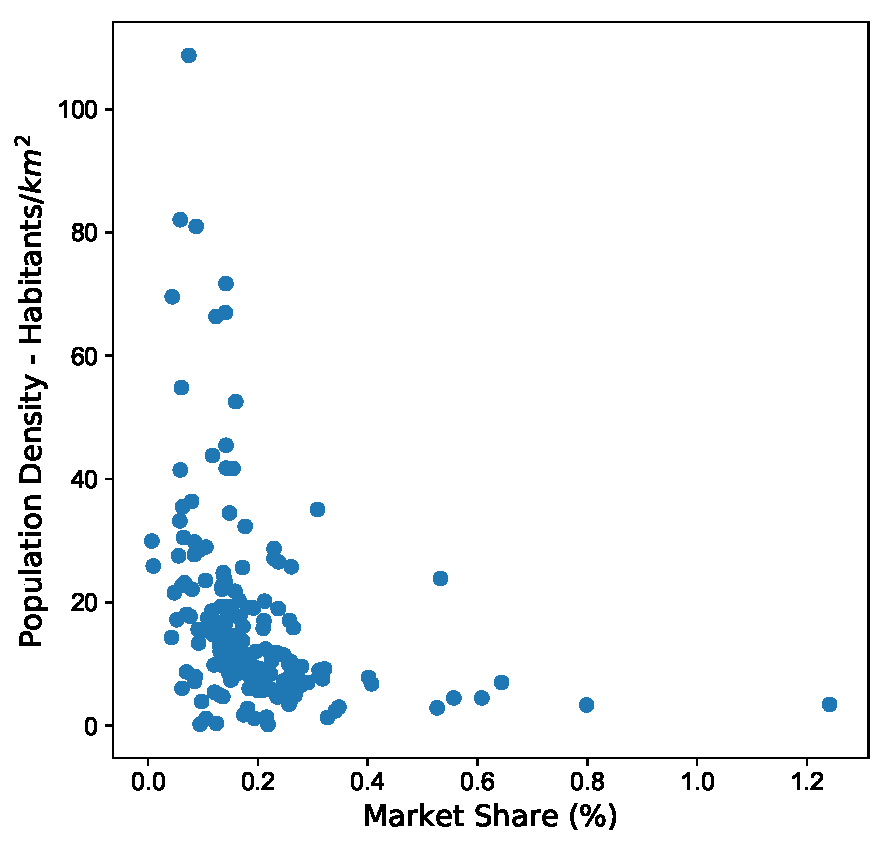
\includegraphics[width=.5\linewidth]{figures/marketShareDensity.pdf}
\caption{Correlation between market share and population density.}
\label{fig:mshare}  
\end{figure}

In~\figurename~\ref{fig:mshare} we report the correlation scatterplot of the market share and the population density. We can see that there is not a clear correlation between the market share and the population.  We can see some outliers: the city with a market share greater than 100\% is the city \emph{Appenzell} that has a very law tax on the car insurance. This is why we have more insurance contracts than inhabitants. On the other city, the city with the larger population is Zurich. We thank the reviewer because it was our mistake to make the aforementioned assumption and this is why we removed it in the revised manuscript. 

At the same time, we believe that the market share feature is representative information because even if, the insurance company la Mobiliere is a national company, is not used equally across the Swiss country. Given the fact, that having an insurance contract is mandatory also for renting an apartment, the information of the market share of a given company can tell us important information about a certain kind of population living in that area. 


\textbf{5. Table 6 and the corresponding discussion in the results give primacy to the statistical significance (p-value) and doesn't make any reference to effect sizes. While statistical significance is obviously important (Within limits. I didn't bother with the exact p-values beyond the annotated ranges),  I find the analysis incomplete without a discussion of the effect direction and sizes and the corresponding implications. In addition, this would have improved the clarity of the results section substantially. At the moment, the authors employ the expressions "strongly connected", "related" etc. when describing relationships between features and socio-economic indicators, but it is not clear whether they are referring to the statistical significance or coefficient sizes and the reader is left to imagine plausible relationships.}
\\
We thank a lot the reviewer for this point that is really important and it was not really clear what was the meaning of Table 6. Table 6 was the table related to the importance of the features in the features selection. We removed that table and we added a table with p-values and   the confidence intervals of the features for the SLM and GWR models. We also discussed the table in the Results section where we show the outcome and the performance of the different models. The new tables are Table 6 and Table 7 in the manuscript. 


\textbf{6. Figures 3(c) and 3(d) that are mentioned in the results section are missing}

We thank a lot the reviewer for this comment. We changed Figure and we mention all the subfigures in the manuscript.

\textbf{7. The discussion on the issue of training the models on regions with widely varying sizes is not clear. First, the authors argue that the training and testing on cities with such variation in size affects performance. Then the authors use a cross-validation approach that stratifies that based on the populations to "cope with this effect". This is followed by a statement that "as expected" general performance declines. May be what the authors meant to say was that they were trying to quantify the effect of applying a model that was trained on some set of municipalities with comparable populations to another one?. The narrative wouldn't make sense if they mean to say that they were solving the problem of "training on cities with different populations" with their stratified cross-validation method since it in fact decreases performance from the original.}

We thank a lot the reviewer again for this point we extensively revised our manuscript in many parts in order to make all of this points more clear. 

\textbf{8. The authors should try to extend their preliminary analysis on model performance across different municipalities more systematically instead of relying largely on anecdotes. Even as it is, I find this analysis adds some novelty and nuance I don't often see in similar work. A systematic exploration would require identification of some pertinent variables along which performance can be evaluated. Many of the dependent variables would be a good place to start; For example, do the models fare better in larger cities or smaller ones? More wealthy ones or poorer ones? Cities where the insurance company has a larger market share or smaller one? etc. Answering these questions would be very useful to understand the nuances of using some predictions in practical contexts like policymaking.}

We thank a lot the reviewer for this comment. We tried to make some analysis in this but we did not find any interesting correlations as shown in the following and also in Section 8.4 of the available notebook.. In~\figurename~\ref{fig:ppop} we show the correlation between the local $R^2$ and the population size for different cities, in~\figurename~\ref{fig:pmshare} the correlation with the market share and in~\figurename~\ref{fig:popdens} the correlation with the population density.

In order to validate our modus operandi we also checked the stability of the feature selection method as reported in Table~\ref{tab:stability} and in  Section 4.1 of the available notebook.

\begin{table}[h!]
\centering
\caption{Stability of the features selection for each target variables.}
\label{tab:stability}
\begin{tabular}{cc}
\hline
 Variable  & Stability \\
\hline

p1& 0.824617\\
p2& 0.690959\\
t1& 0.571393\\
t2& 0.779439\\
w1& 0.700473\\
w2& 0.714200\\
s1& 0.544287\\
s2& 0.603708\\
h1& 0.414831\\
h2& 0.720396\\
e1& 0.247062\\
e2& 0.655891\\
\end{tabular}
\end{table}

From the table above we can see the target variables we are able to predict well are also the ones that have high stability in terms of feature selection. On the other side variable like $e_2$ are not well predicted and also the features selection is completely random.

\begin{figure}[h!]
    \centering
    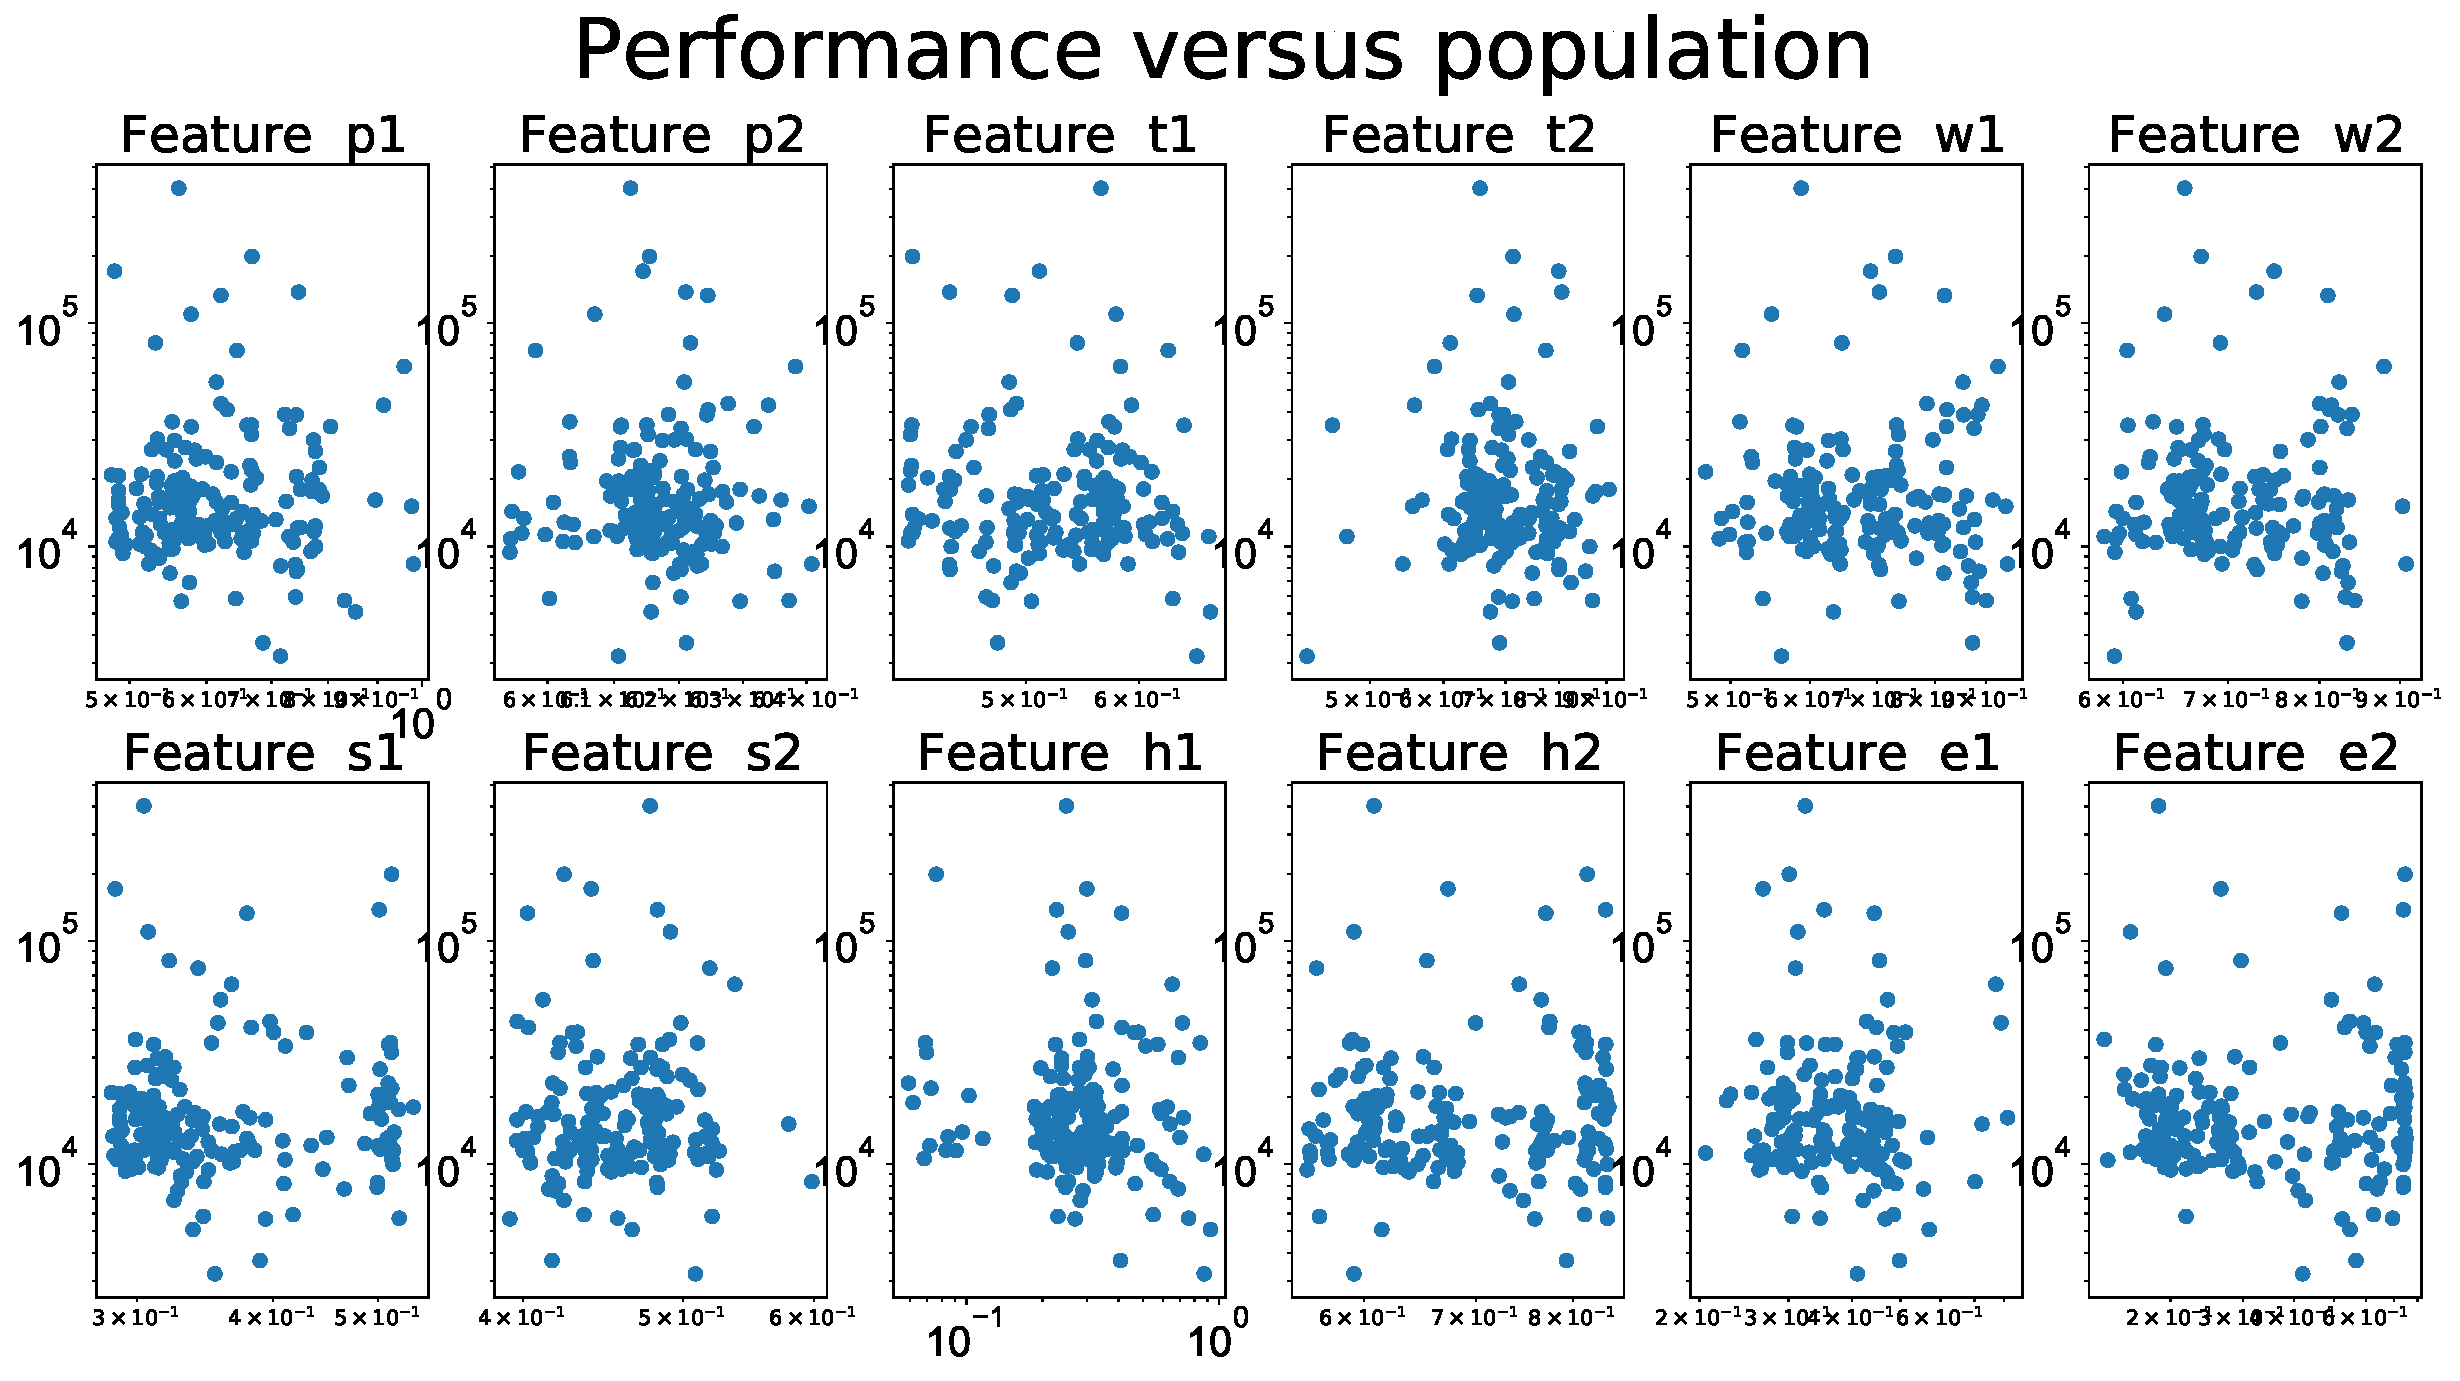
\includegraphics[width=1\linewidth]{figures/ppop.pdf}
\caption{Correlation between local $R^2$ and population size.}
\label{fig:ppop}  
\end{figure}

\begin{figure}[h!]
    \centering
    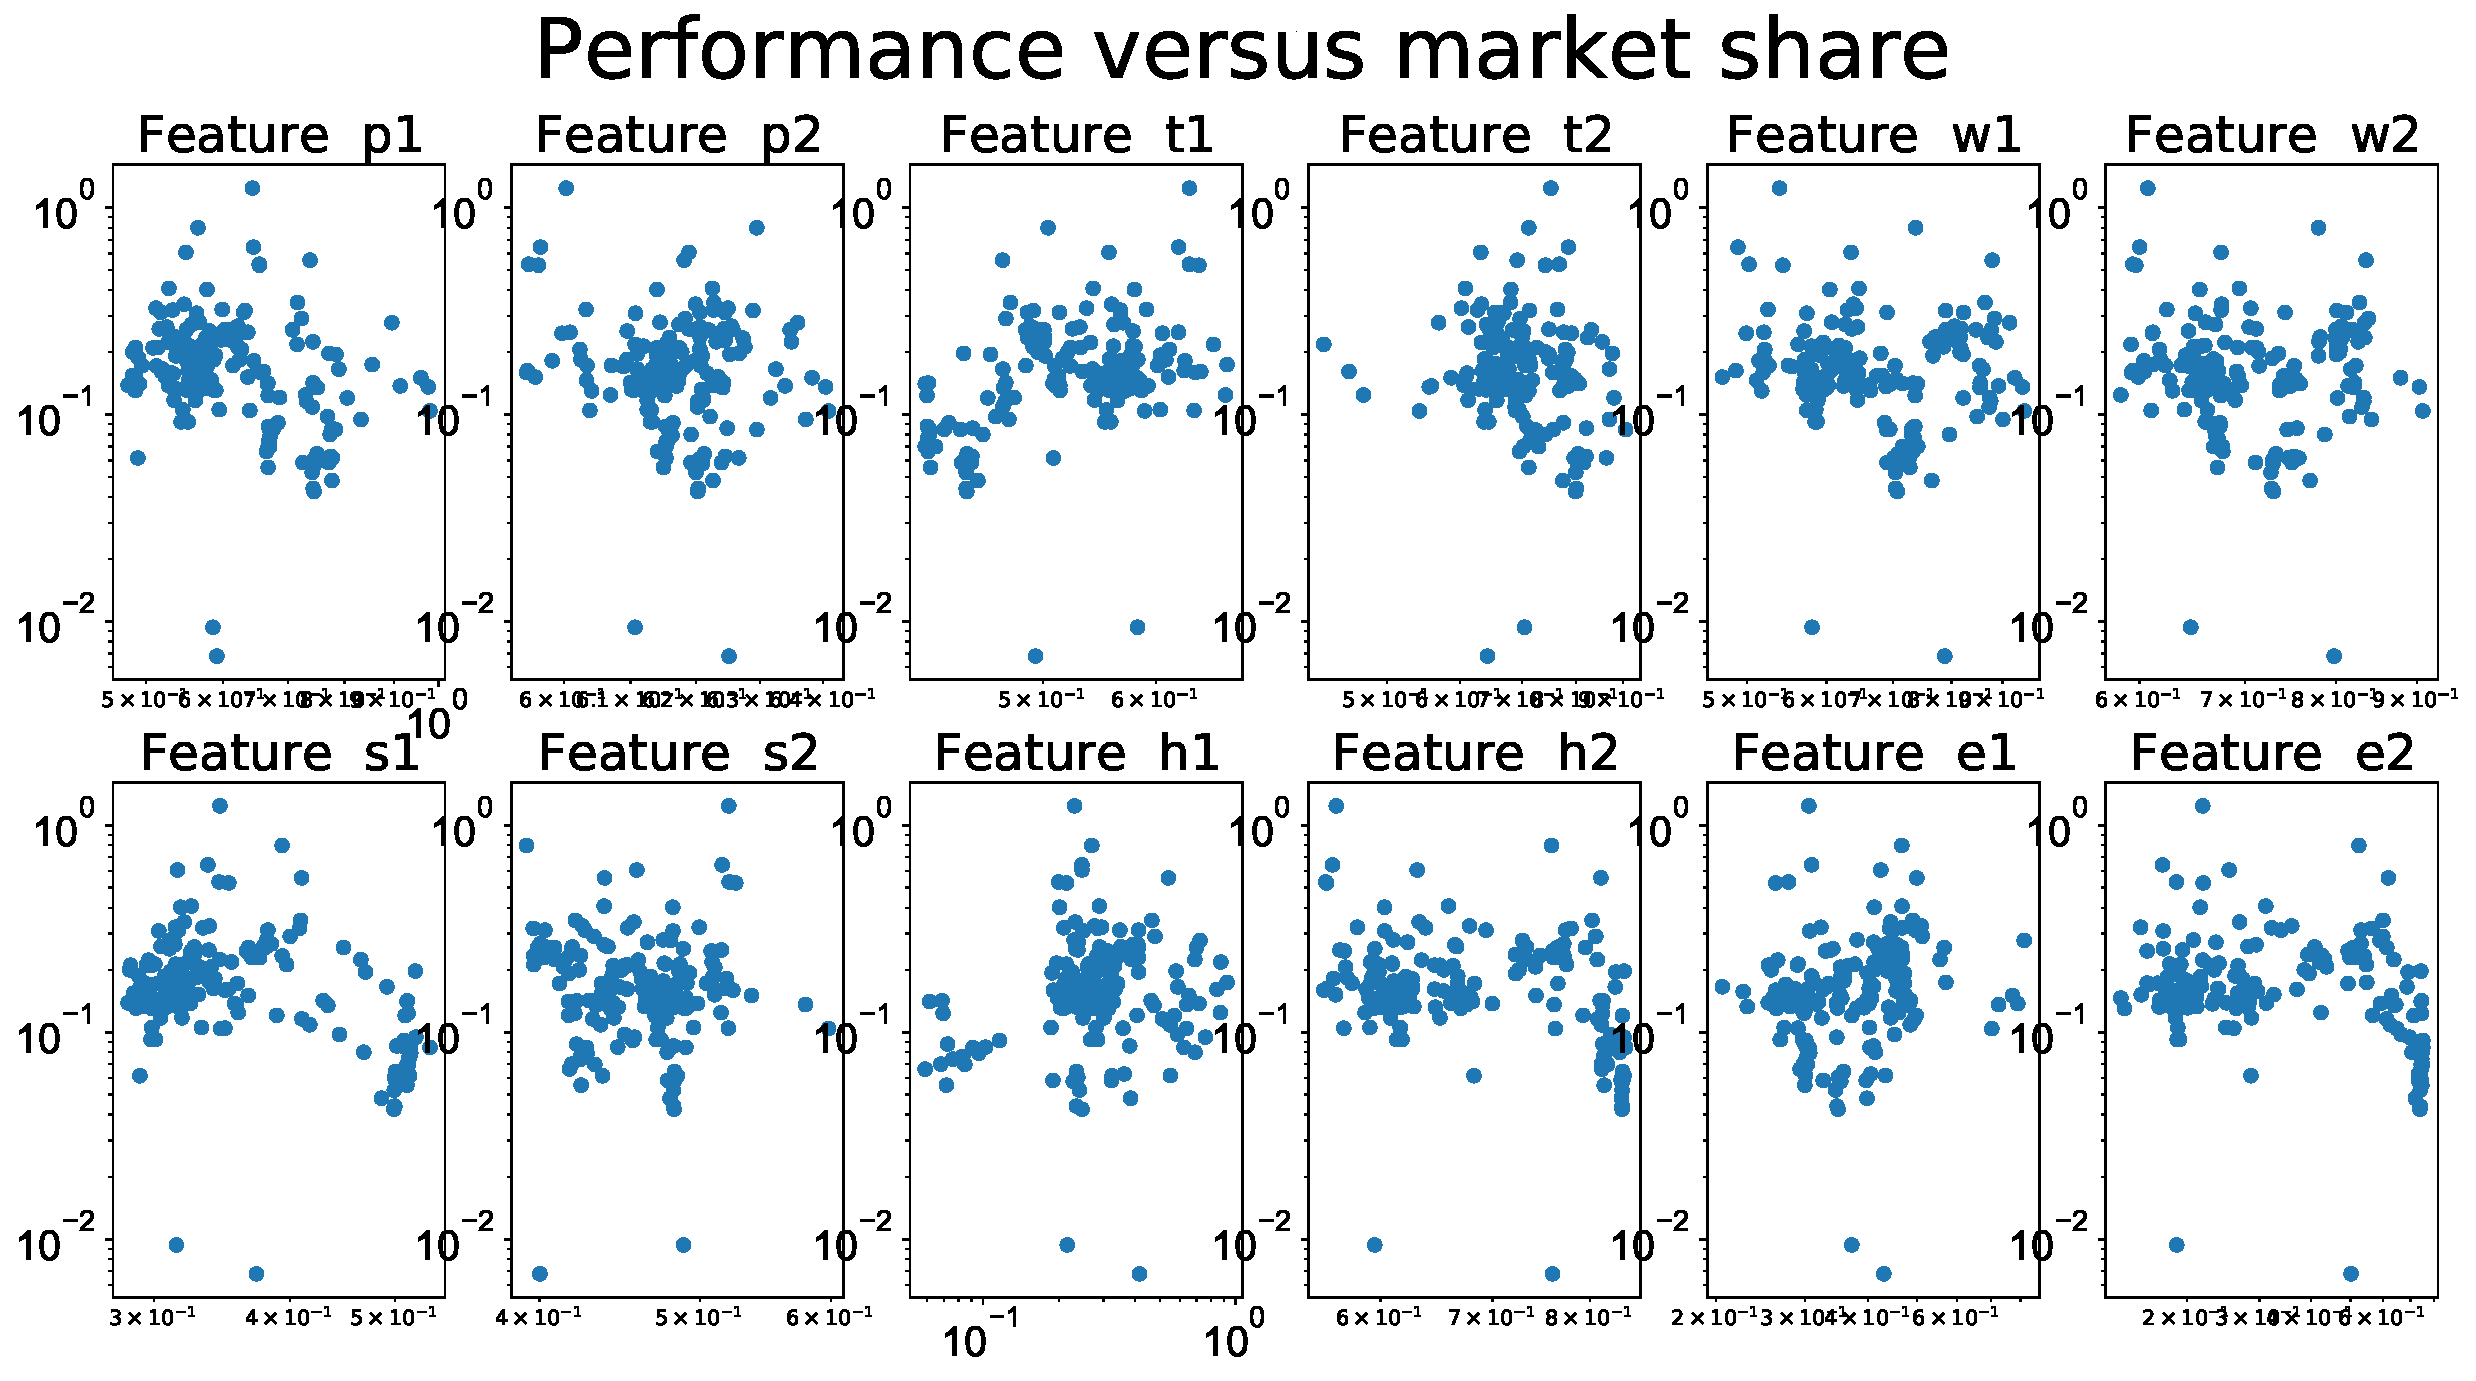
\includegraphics[width=1\linewidth]{figures/pmshare.pdf}
\caption{Correlation between local $R^2$ and market share.}
\label{fig:pmshare}  
\end{figure}

\begin{figure}[h!]
    \centering
    \includegraphics[width=1\linewidth]{figures/popdens.pdf}
\caption{Correlation between local $R^2$ and the population density}
\label{fig:popdens}  
\end{figure}




\clearpage
\bibliography{scibib}
\bibliographystyle{Science}


\end{document}




















